%
% @file slides_cz.tex
% @author David Kvaček (xkvace00@stud.fit.vutbr.cz)
% @brief Source code of the LaTeX bachelor's thesis presentation.
% @date 2025-06-17
%

\begin{frame}
  \frametitle{Motivace a~cíle práce}
  \begin{columns}
  \column{0.42\textwidth}
    \begin{itemize}
      \item Plánování \emph{sportovních}\\aktivit a~výkonů
      \bigskip
      \item Analýzy a~grafické\\\emph{vizualizace}
    \end{itemize}

  \column{0.58\textwidth}
    \centering\includegraphics[width=\textwidth]{img/wfcc7_06_1.jpeg}
  \end{columns}
\end{frame}

\begin{frame}
  \frametitle{Použité technologie a~architektura nástroje}
  \begin{columns}
  \column{0.36\textwidth}
    \begin{itemize}
      \item \emph{Multiplatformní} řešení\\(framework Flutter)
      \bigskip
      \item Architektura \emph{klient--server}\\(framework FastAPI)
      \bigskip
      \item \emph{Geografická} data různých formátů
    \end{itemize}

  \column{0.64\textwidth}
    \centering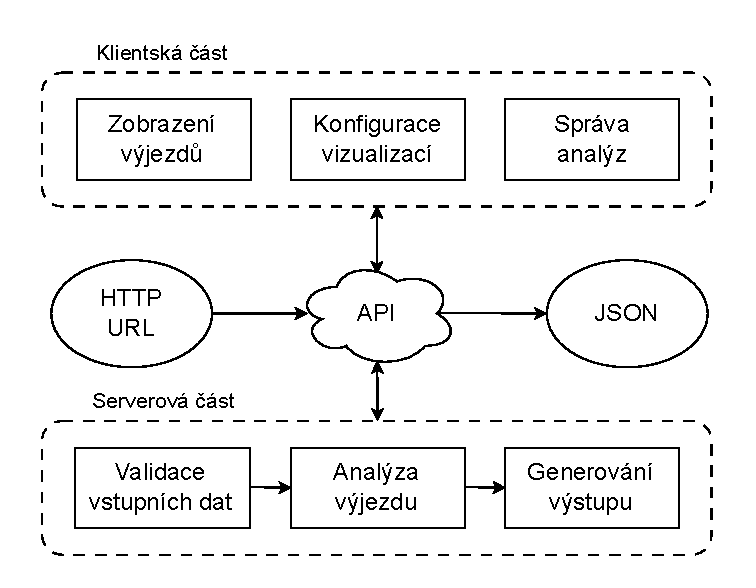
\includegraphics[width=\textwidth]{img/architecture.pdf}
  \end{columns}   
\end{frame}

\begin{frame}
  \frametitle{Výpočet vzdálenosti a~sklonu stoupání}
  \begin{columns}
    \column{0.50\textwidth}
      \centering\includegraphics[width=0.48\textwidth]{img/Illustration_of_great-circle_distance.svg.png}

    \column{0.50\textwidth}
      \centering
\includegraphics[width=0.86\textwidth]{img/gradient.png}
  \end{columns}

  \bigskip

  \[
    l = 2r \times \arcsin \left( \sqrt{\sin^2\left(\frac{\phi_Q - \phi_P}{2}\right) + \cos(\phi_P) \times \cos(\phi_Q) \times \sin^2\left(\frac{\lambda_Q - \lambda_P}{2}\right)} \right)
  \]

  \[
    c = \frac{b}{a} \times 100\,\%
  \]
\end{frame}

\begin{frame}
  \frametitle{Výstupy aplikace}
  \begin{columns}
  \column{0.40\textwidth}
    \begin{itemize}
      \item Základní a~pokročilé \emph{statistiky} pro porovnávání
      \bigskip
      \item \emph{Vizualizace} tras na mapových podkladech
    \end{itemize}
  \column{0.60\textwidth}
    \centering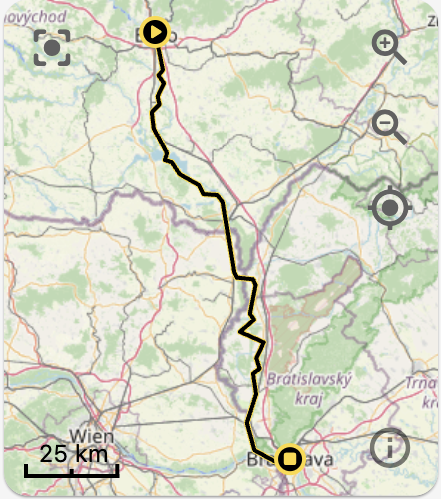
\includegraphics[width=0.64\textwidth]{img/map.png}
  \end{columns}
\end{frame}

\begin{frame}
  \frametitle{Výstupy aplikace}
\begin{tikzpicture}
    \node[inner sep=0pt] at (0,0) {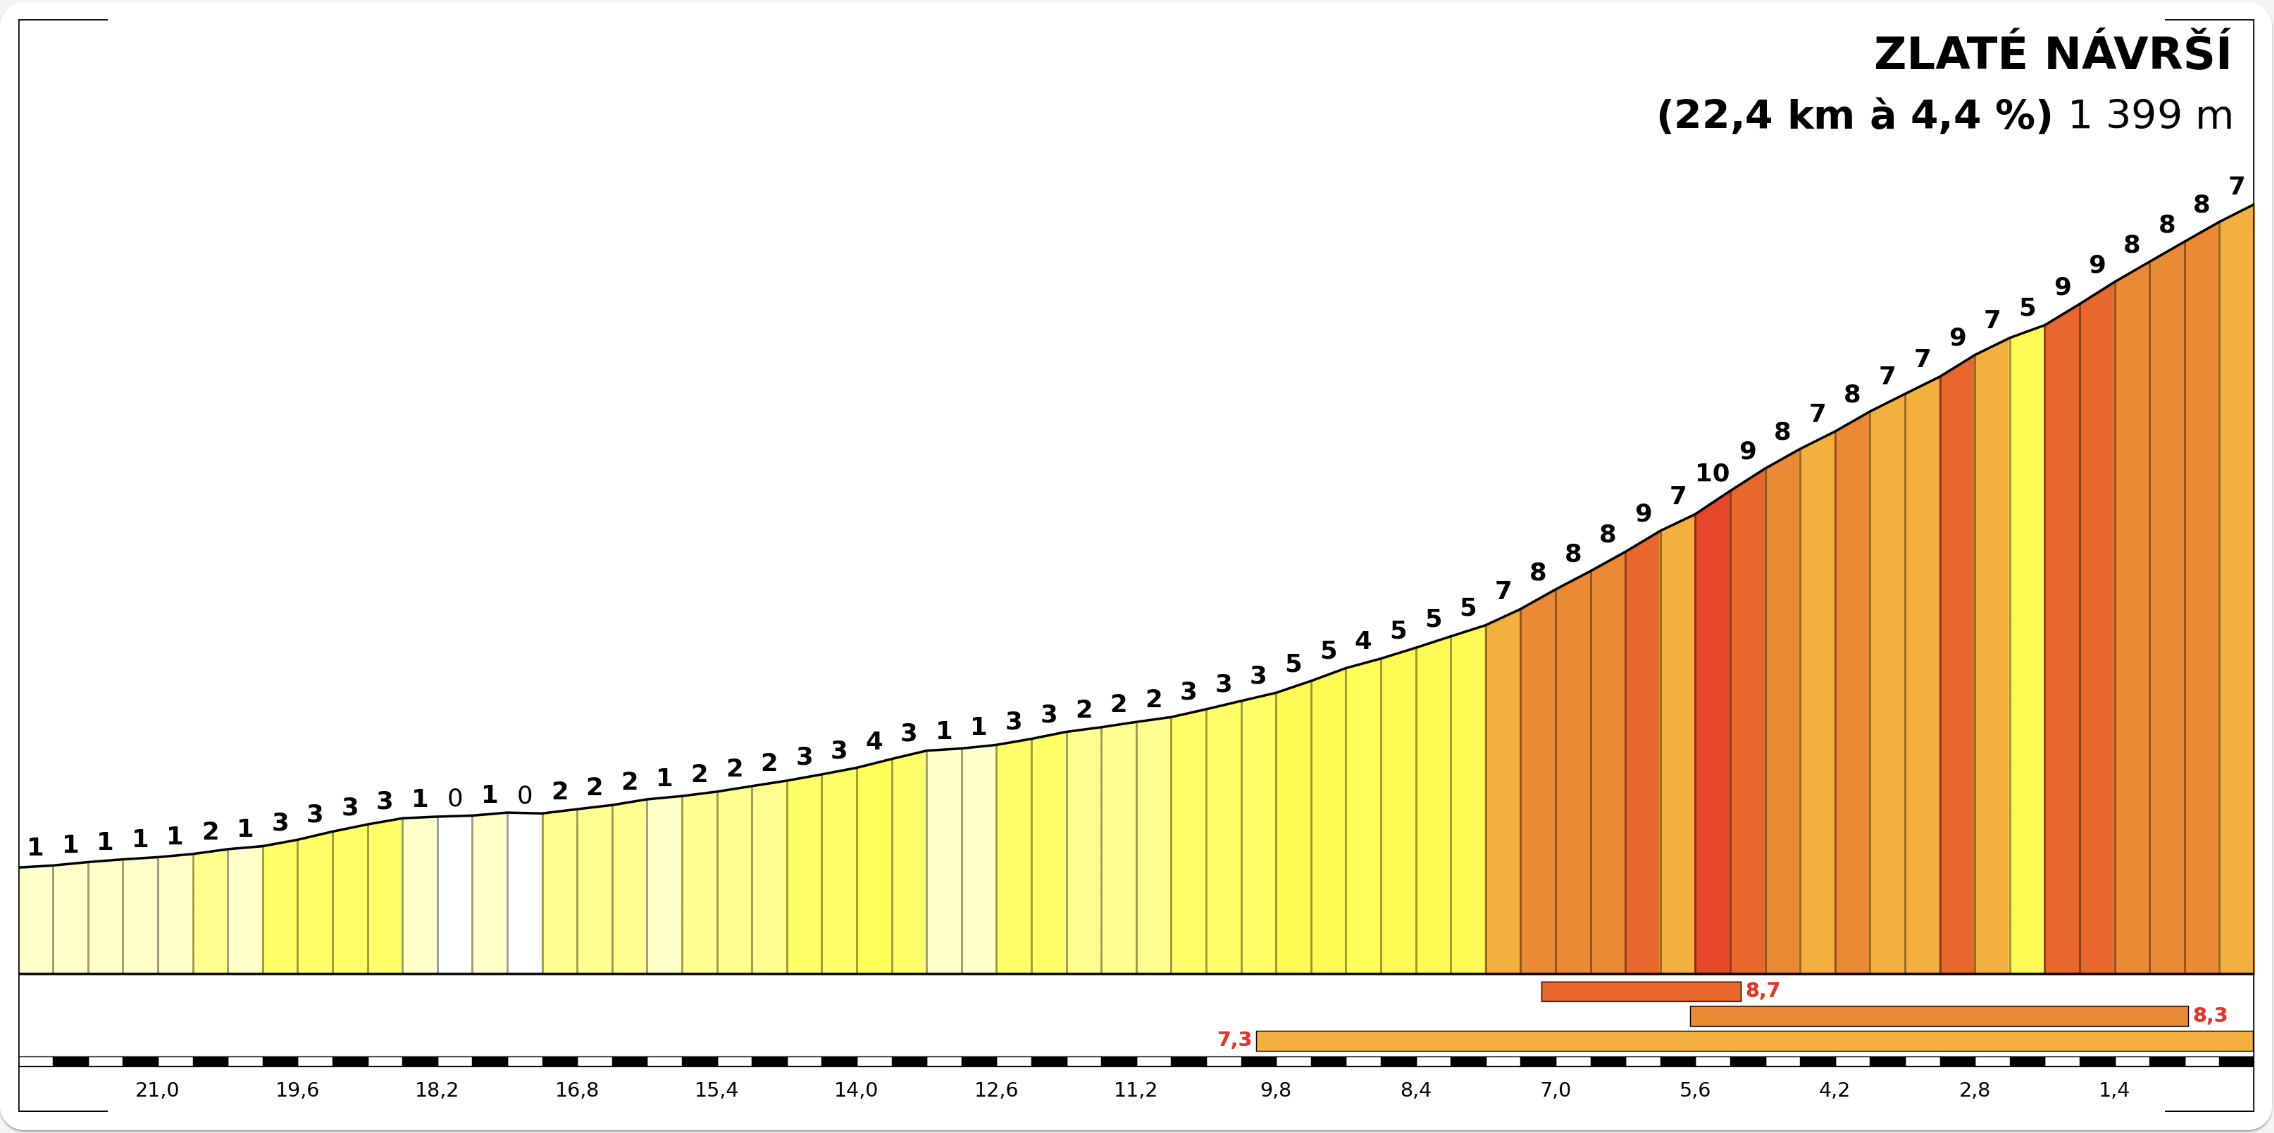
\includegraphics[width=0.64\textwidth]{img/climb-profile.png}};
    \node[inner sep=0pt] at (-5.0cm,3.0cm) {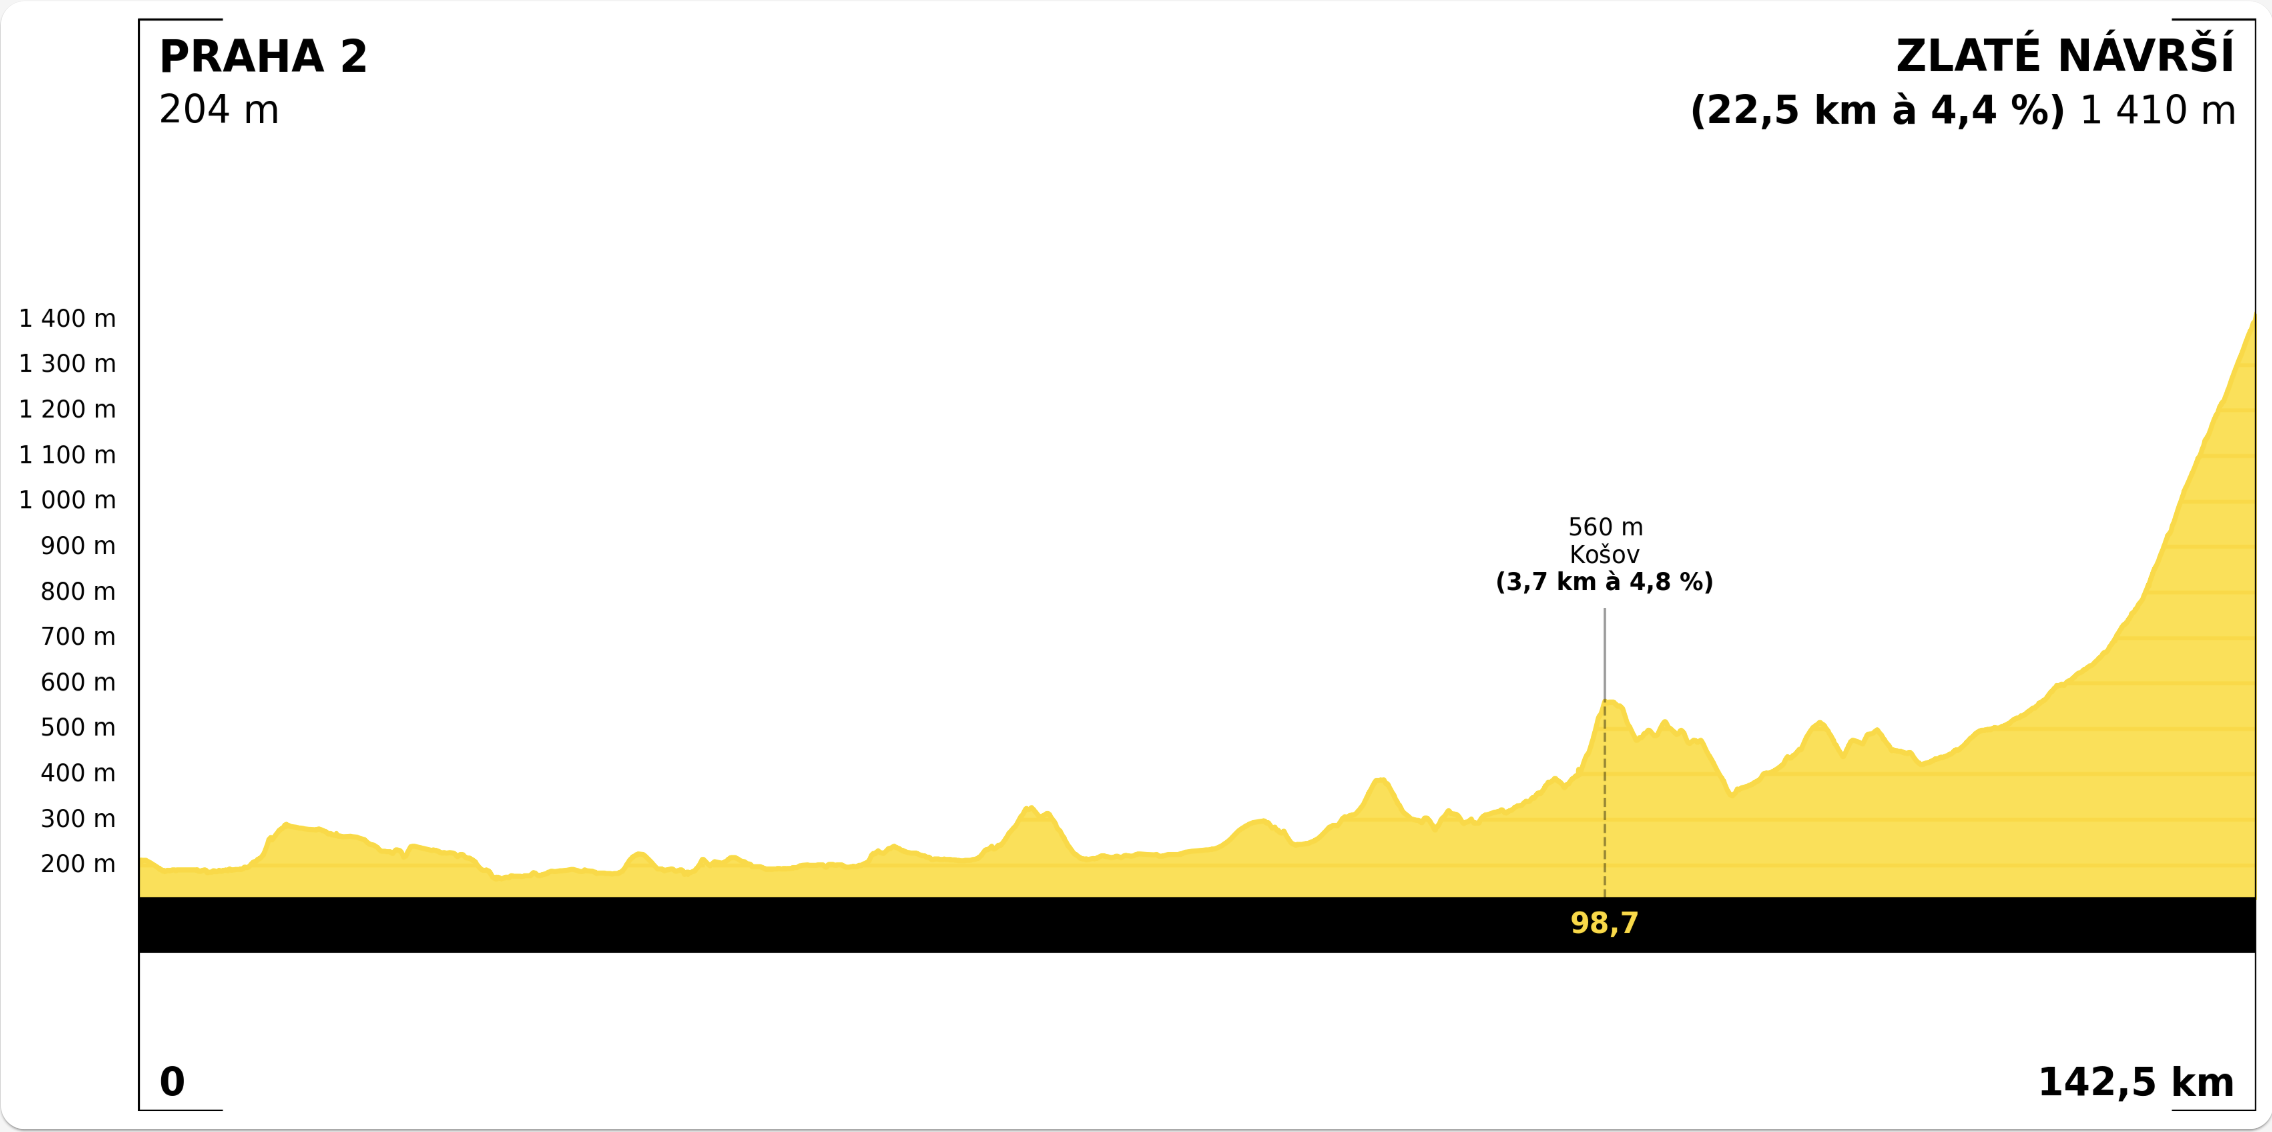
\includegraphics[width=0.64\textwidth]{img/trip-profile.png}};
\end{tikzpicture}
\end{frame}

\begin{frame}
  \frametitle{Děkuji za pozornost!}
  \centering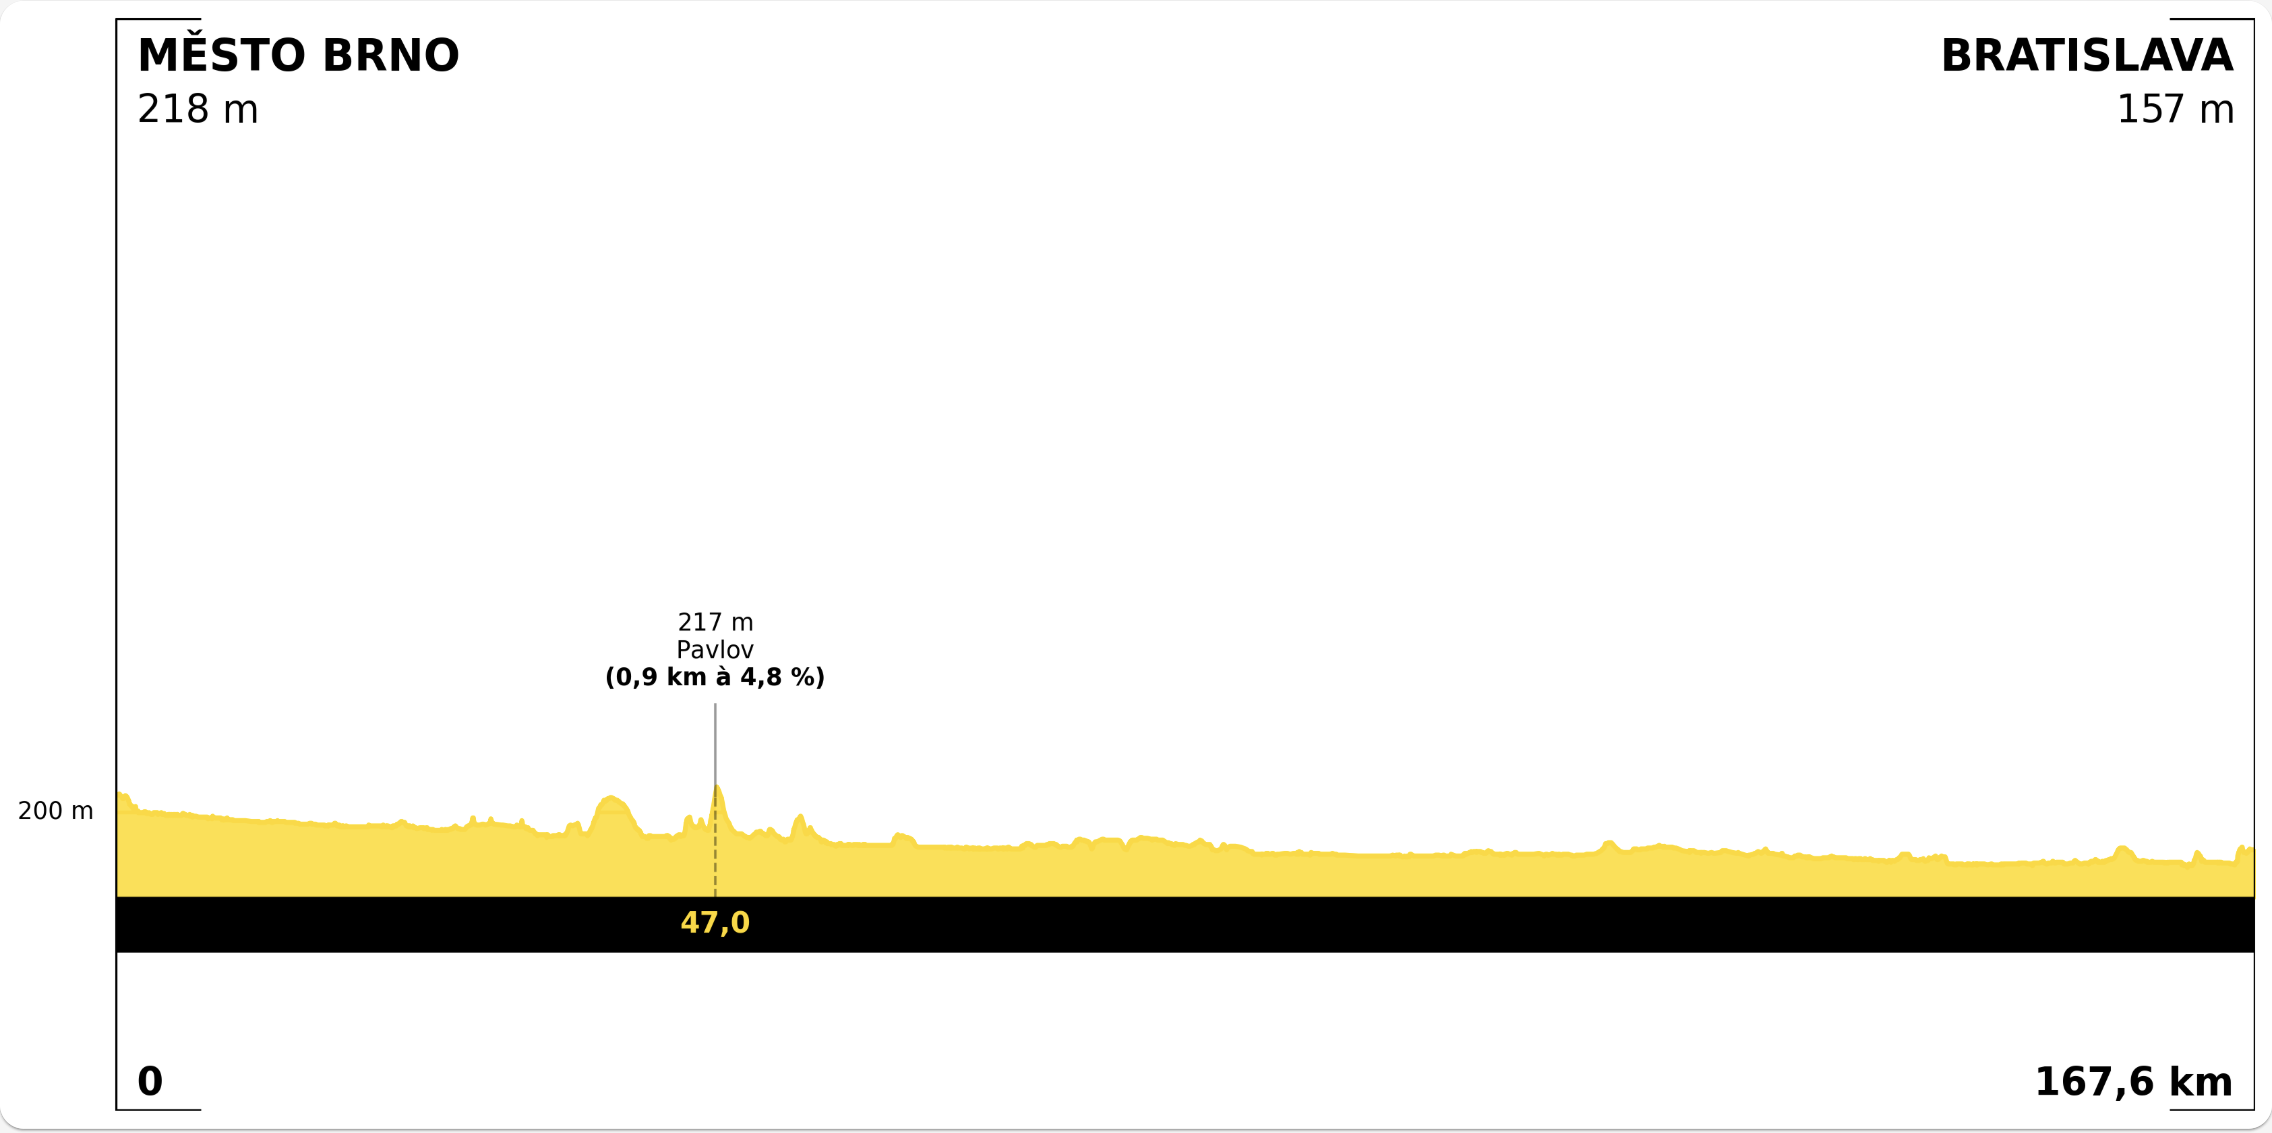
\includegraphics[width=\textwidth]{img/flat.png}
\end{frame}

\appendix{}

\begin{frame}
  \frametitle{Otázky k~obhajobě}
  Bylo by možné do řešení integrovat nějakou mapovou službu (např. Mapy.cz) a~soubory o~trasách si stahovat přímo v~rámci uživatelského plánování?
  \bigskip
  \begin{itemize}
    \item REST API Mapy.cz
    \item Overpass API (OpenStreetMap)
  \end{itemize}
\end{frame}

\begin{frame}
  \frametitle{Otázky k~obhajobě}
  Průměrná rychlost celé trasy je uživatelsky definovaná. Šlo by ji nějak předpovídat pro jednotlivé části trasy?
  \bigskip
  \begin{itemize}
    \item Dílčí vzdálenost
    \item Průměrný sklon
    \item Index obtížnosti
  \end{itemize}
\end{frame}

\begin{frame}
  \frametitle{Otázky k~obhajobě}
  Plánujete řešení nasadit pro veřejnost?
  \bigskip
  \begin{itemize}
    \item Spuštění serverové části
    \item Nasazení webové stránky
  \end{itemize}
\end{frame}
